\documentclass{beamer}
\usetheme{Frankfurt}

\usepackage{listings}

\newcommand{\todo}[1]{\alert{TODO #1}}

\title{Networking/OS}
\subtitle{Lecture 2 \\ Computer Security DD2395}
\author[R. Guanciale]{
  Roberto Guanciale\\
  robertog@kth.se
}
\date{2015-11-04}
\begin{document}

\begin{frame}[plain]
  \titlepage
\end{frame}

\begin{frame}{Outline for Today}
  \begin{itemize}
    \item Computer networking
    \item Operating systems
  \end{itemize}
\end{frame}

\begin{frame}{Introduction to IP networking}
  \begin{itemize}
    \item An end host requests a web-page from a server via a local-area
      network
    \item The aim of this lecture is to give an overview of how this works
in practice
  \end{itemize}
  \begin{center}
    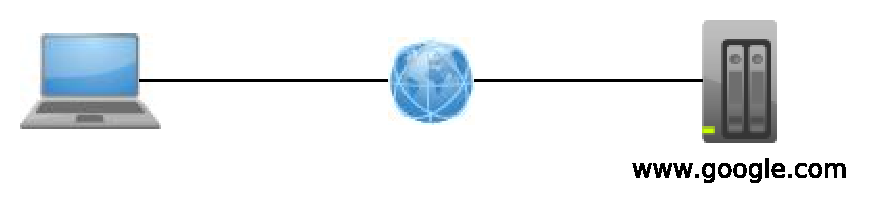
\includegraphics[width=0.5\linewidth]{net0}
  \end{center}
\end{frame}

\begin{frame}{Introduction to IP networking}
  Every routing domain is independently administrated
  \begin{center}
    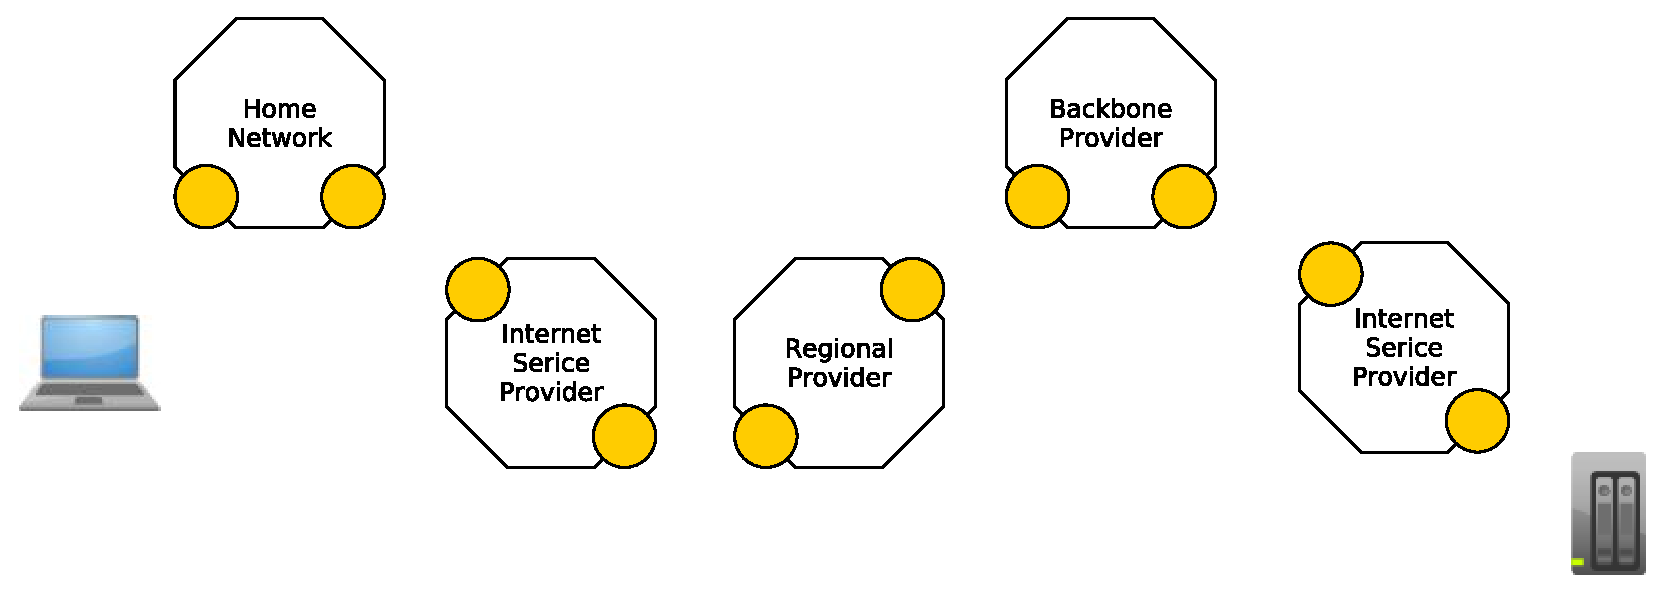
\includegraphics[width=0.8\linewidth]{net1}
  \end{center}
\end{frame}

\begin{frame}{The Hourglass Model}
  \begin{itemize}
    \item Anything over IP – IP over anything
    \item All applications depend on IP
    \item IP runs over all networks
    \item IP is at the heart of all communicati
  \end{itemize}
  \begin{center}
    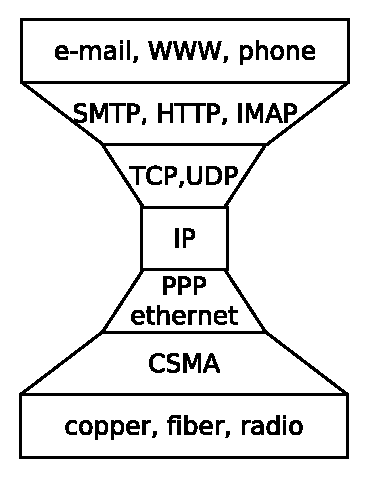
\includegraphics[width=0.4\linewidth]{net2}
  \end{center}
\end{frame}

\begin{frame}{Stack}
  \begin{center}
    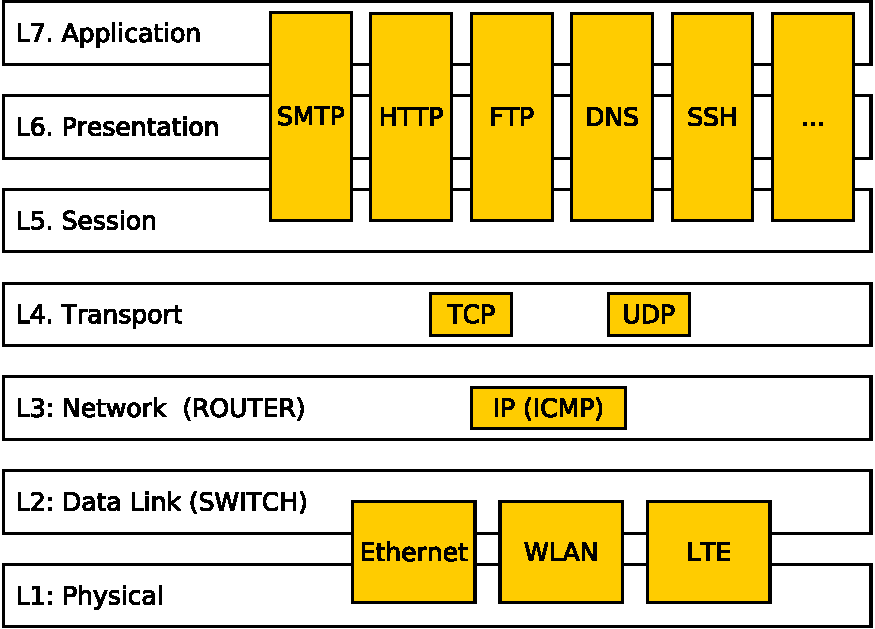
\includegraphics[width=0.4\linewidth]{stack}
  \end{center}
\end{frame}

\begin{frame}{Encapsulation}
  \begin{center}
    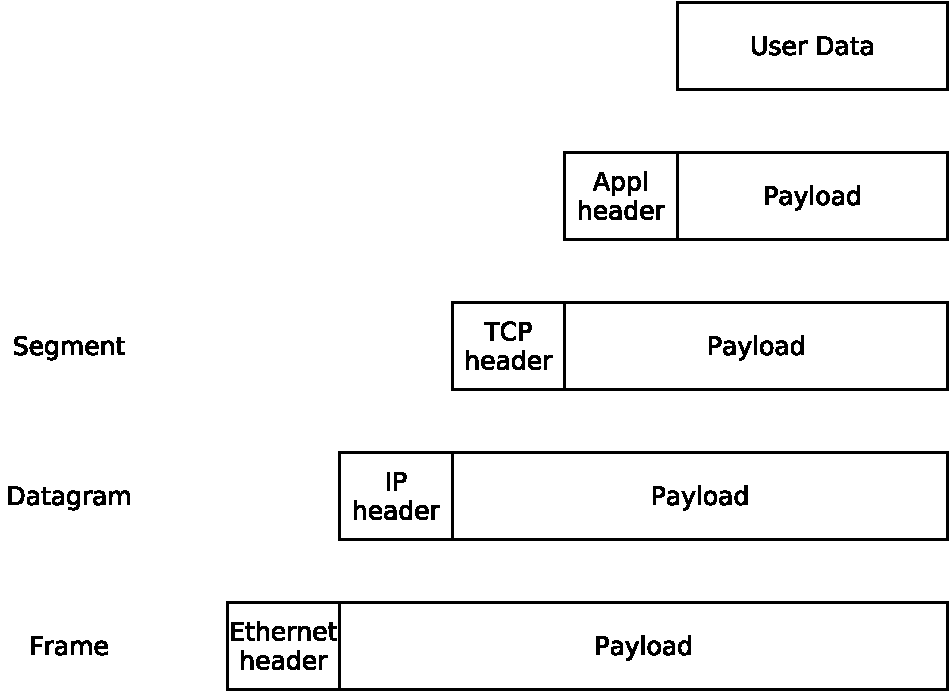
\includegraphics[width=0.7\linewidth]{encapsulation}
  \end{center}
\end{frame}

\begin{frame}
  \begin{itemize}
  \item Using a link-level protocol, you can now communicate
    directly over a link
  \item The network layer (IP) primarily adds the ability to cross
    several networks using 'routing'
  \item Each interface in an IPv4 Internet is assigned a unique 32-bit
internet address (Not node addresses!)
  \begin{itemize}
\item Address types
\item Unicast – one-to-one
\item Anycast - one-to-any
\item Multicast – one-to-many
\item Broadcast – one-to-all
  \end{itemize}
\item Notation, dotted-decimal: 192.36.125.18
\item An address has two purposes
  \begin{itemize}
\item Netid (prefix) identifies a network
\item Hostid identifies a node on that network
  \end{itemize}
\item Slash notation: 192.36.120.0/21
  \end{itemize}
\end{frame}

\begin{frame}{IP-header}
  \begin{center}
    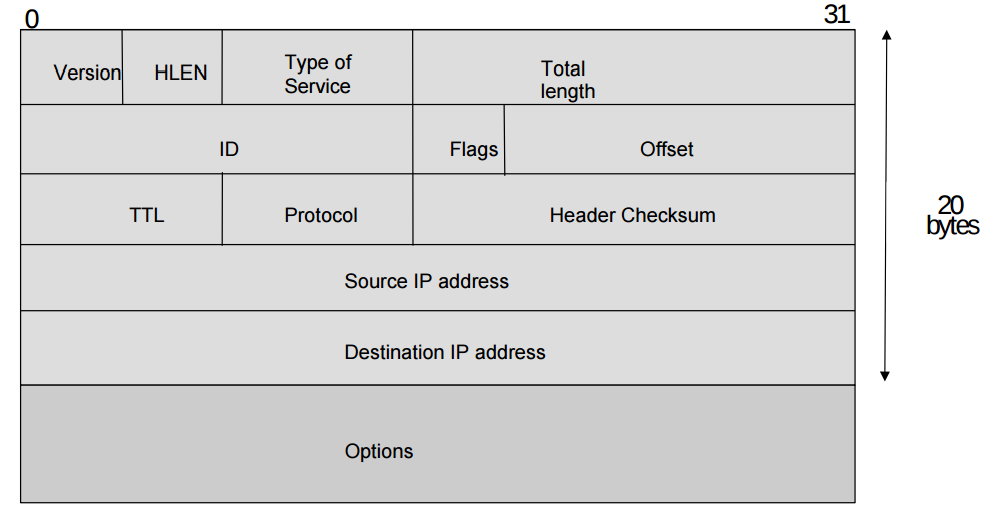
\includegraphics[width=0.9\linewidth]{IP-header}
  \end{center}
\end{frame}

\begin{frame}{IP-routing}
  \begin{center}
    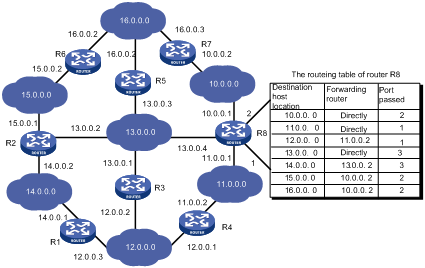
\includegraphics[width=0.9\linewidth]{table}
  \end{center}
\end{frame}

\begin{frame}{ICMP}
  \begin{itemize}
  \item ICMP is a limited signalling protocol for IPv4.
  \item Report IP problems back to sender
  \item Control and Management
  \item 0 - Echo reply (used to ping)
  \item 3 - Destination Unreachable
  \item 8 - Echo request (used to ping)
  \item 9 - Router Advertisement
  \item 11 - Time Exceeded[
  \item 13 - Timestamp
  \item 14 - Timestamp Reply
  \item \dots
  \end{itemize}
\end{frame}

\begin{frame}{Transport layer}
  \begin{itemize}
  \item Provides service to end-applications: ports
  \item UDP
    \begin{itemize}
      \item Packet-oriented
      \item Unreliable
      \item Full-duplex
      \item Data in packets
      \item Real-time traffic/Reliability in application
    \end{itemize}
  \item TCP
    \begin{itemize}
      \item Connection-oriented
      \item Reliable
      \item Full-duplex
      \item Data as byte-stream
      \item Mostly used
    \end{itemize}
  \end{itemize}
\end{frame}

\begin{frame}{UDP}
    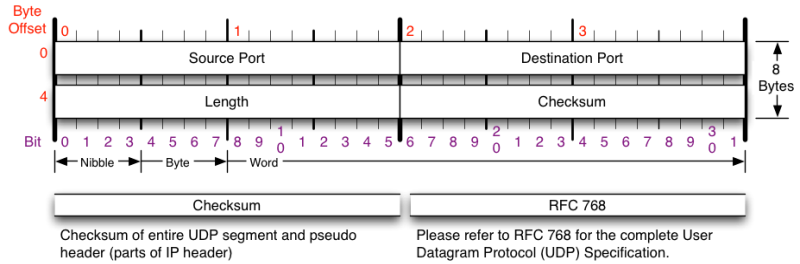
\includegraphics[width=0.9\linewidth]{udp}
\end{frame}

\begin{frame}{TCP}
    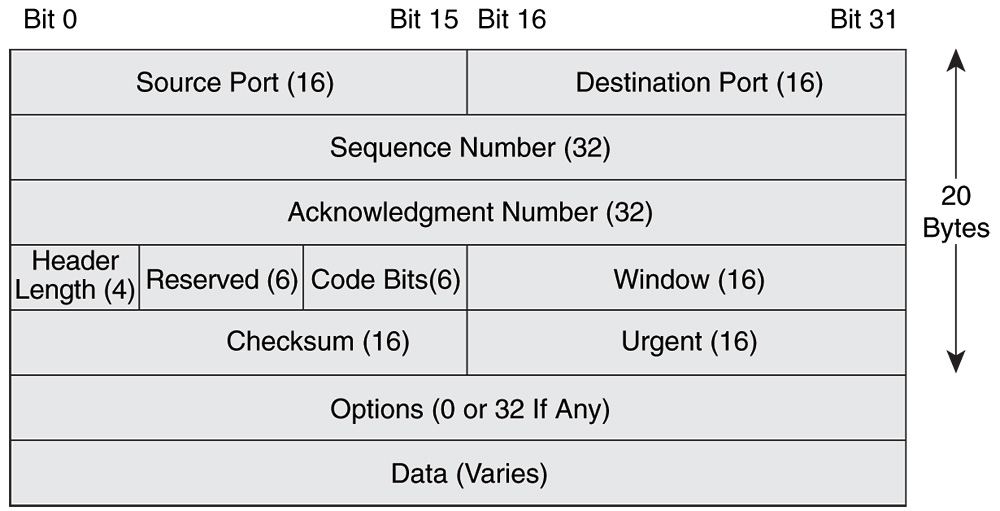
\includegraphics[width=0.9\linewidth]{tcp}
\end{frame}

\begin{frame}{TCP}
    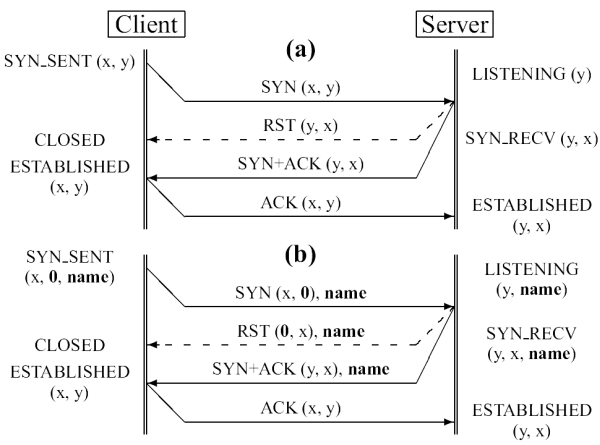
\includegraphics[width=0.7\linewidth]{synack}
\end{frame}

\begin{frame}{DNS}
\begin{itemize}
  \item Why do we need names?
  \item In the underlying network and transport layers it is all about
addresses.
\item Names are better for humans\\
fe80::216:d3ff:fecc:c00d
\item Names add another layer of indirection
\begin{itemize}
\item One name can map to several logical addresses
\item One logical adress can map to several names
\item Names can be used for other things than just addressing
  load balancing, mail direction, descriptions, finding services,
\end{itemize}
\end{itemize}
\end{frame}

\begin{frame}{DNS architecture}
\begin{itemize}
  \item Names are structured hierarchically - in a tree form
  \item The DNS architecture is client-server
\begin{itemize}
\item Client is called resolver
\item Server is called name server
\end{itemize}
\item The resolver queries the nameservers hierarchically
\item Protocol over UDP
\end{itemize}
\end{frame}

\begin{frame}{SMTP}
    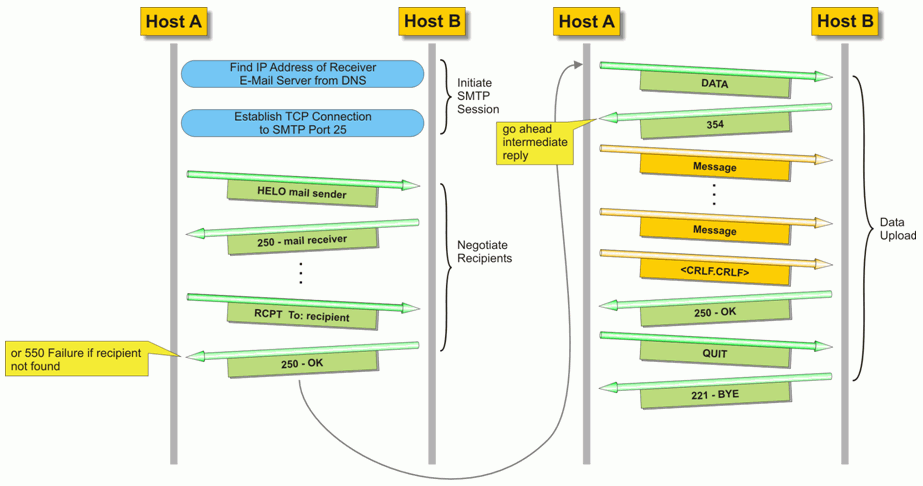
\includegraphics[width=0.7\linewidth]{smtp}
\end{frame}
\begin{frame}{SMTP}
    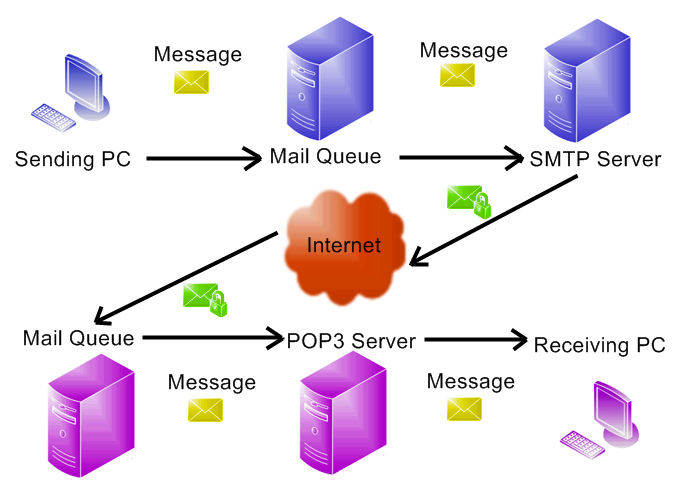
\includegraphics[width=0.7\linewidth]{smrp_queue}
\end{frame}
\begin{frame}{SMTP}
    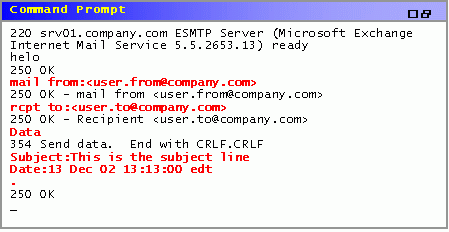
\includegraphics[width=0.7\linewidth]{smtp_shell}
\end{frame}
\begin{frame}{HTTP}
    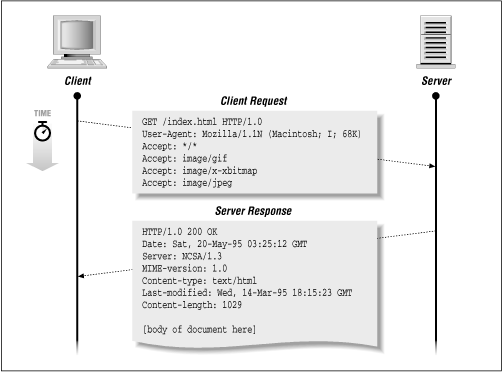
\includegraphics[width=0.7\linewidth]{http}
\end{frame}

\begin{frame}{Questions?}
    Questions?
\end{frame}

\begin{frame}{Operating Systems}
  \begin{itemize}
  \item An OS is a program that acts an intermediary
    between the user of a computer and computer
    hardware
  \item Major cost of general purpose computing is
    software
  \item OS simplifies and manages the complexity of running
    application programs efficiently
  \end{itemize}
\end{frame}

\begin{frame}{Goals of OS}
  \begin{itemize}
  \item Simplify the execution of user programs and
    make solving user problems easier.
  \item Allow sharing of hardware and software resources.
  \item Make application software portable and versatile.
  \item Provide isolation, security and protection among
    user programs.
  \end{itemize}
\end{frame}

\begin{frame}{Example of OSes}
  \begin{itemize}
  \item Windows/Linux/OS X ($\sim$ 50 milions LOC)
  \item<2-> Android/iOS ($\sim$ 50 milions LOC)
  \item<3-> S40 ($\sim$ 1 milions LOC)
  \item<4-> Free RTOS ($\sim$ 10 000 LOC)
  \item<5-> L4 microkernel ($\sim$ 10 000 LOC)
  \item<6-> Automotive
  \item<7-> SCADA
  \end{itemize}
\end{frame}

\begin{frame}{How we run Chrome and Open Office on the same CPU?}
  How we run Chrome and Open Office on the same CPU?
\end{frame}

\begin{frame}{HW architecture}
  \begin{itemize}
  \item Memory
  \item CPU
    \begin{itemize}
    \item Registers (super fast small memory, program counter)
    \item Privilege level (i.e. Ring 3/Ring 0, PL1/PL0, CPU modes)
    \end{itemize}
  \item OS-kernel takes control of privileged level
  \item Everithing else uses non-privileged level
  \end{itemize}
  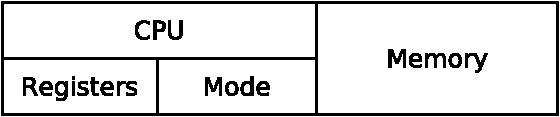
\includegraphics[width=0.5\linewidth]{hw}
\end{frame}

\begin{frame}{Virtual Memory}
  \begin{itemize}
  \item Modern systems do not use directly physical addresses
    \begin{itemize}
    \item Free to allocate applications in different memory area
    \item Free to dynamically allocate memory for processes
    \item Run the same software in systems with 1GB or 2 GB of memory
    \item Run the same binary as two distinct processes
    \end{itemize}
  \item Virtual memory
    \begin{itemize}
    \item SW uses virtual addresses
    \item HW configuration maps virtual addresses to physical addresses
    \item HW configuration updatable
    \item HW configuration are called page tables
    \item HW mechanism is called Memory Management Unit
    \end{itemize}
  \end{itemize}
\end{frame}

\begin{frame}{Virtual Memory}
  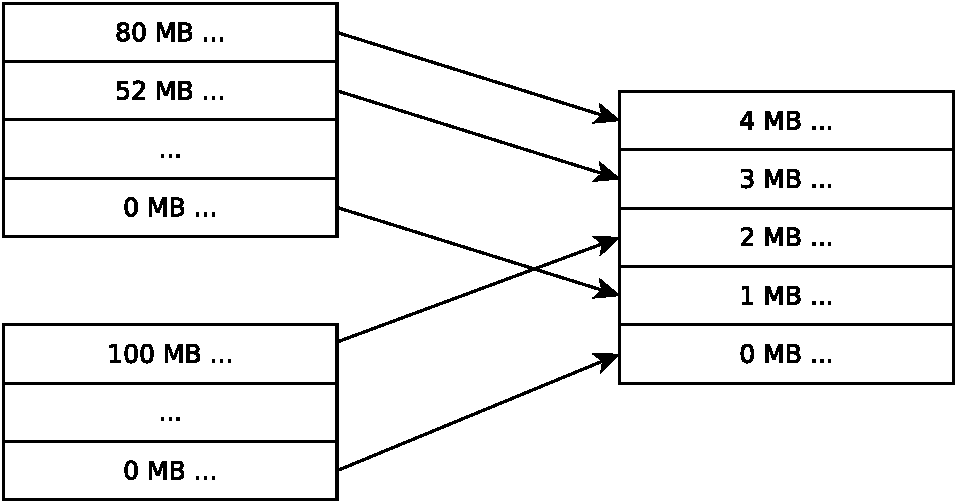
\includegraphics[width=0.8\linewidth]{va2pa}
\end{frame}

\begin{frame}{Virtual Memory}
  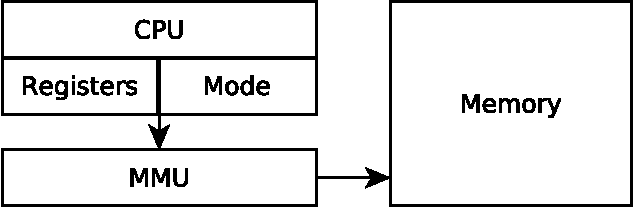
\includegraphics[width=0.8\linewidth]{hw2}
\end{frame}

\begin{frame}{Virtual Memory}
  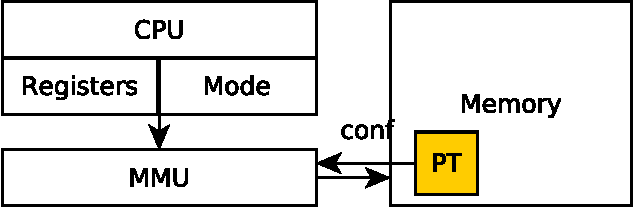
\includegraphics[width=0.8\linewidth]{hw3}
\end{frame}

\begin{frame}{Virtual Memory}
  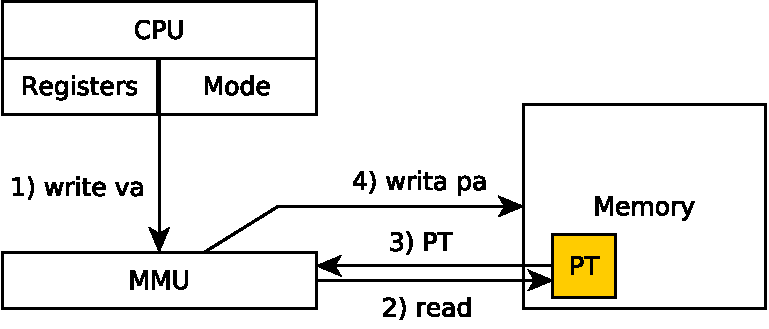
\includegraphics[width=0.8\linewidth]{hw4}
\end{frame}

\begin{frame}{Virtual Memory}
  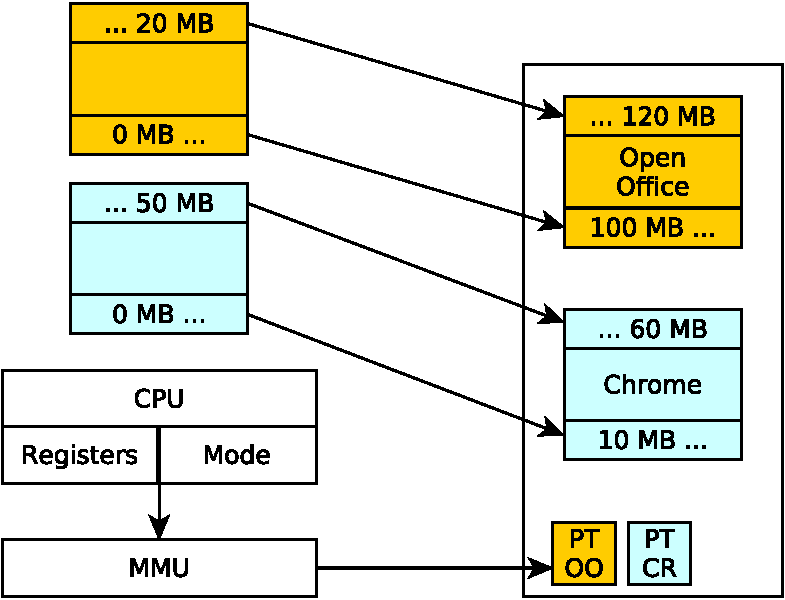
\includegraphics[width=0.6\linewidth]{process}
\end{frame}

\begin{frame}{Virtual Memory}
  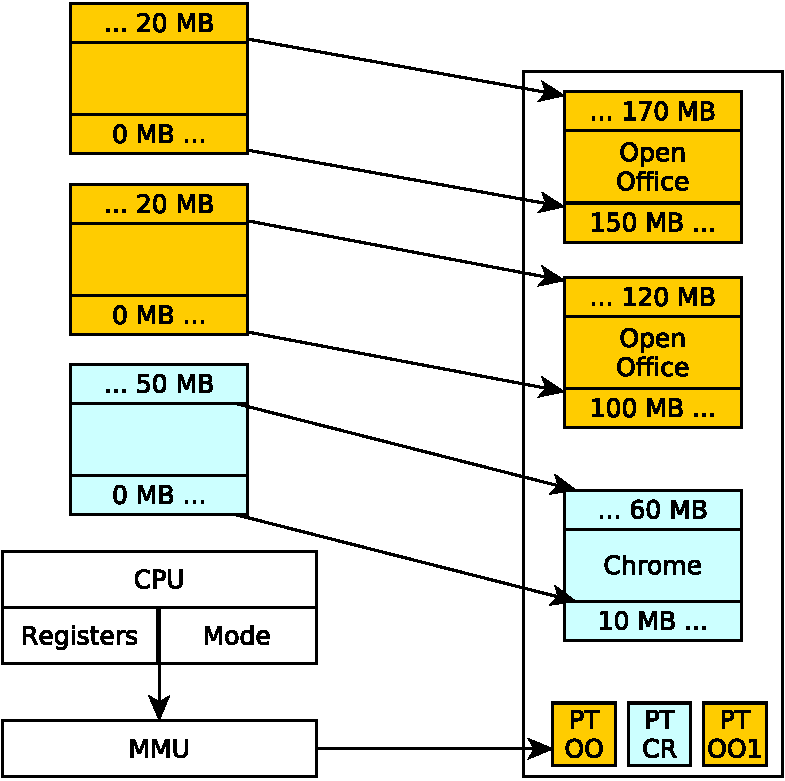
\includegraphics[width=0.6\linewidth]{process1}
\end{frame}

\begin{frame}{Virtual Memory}
  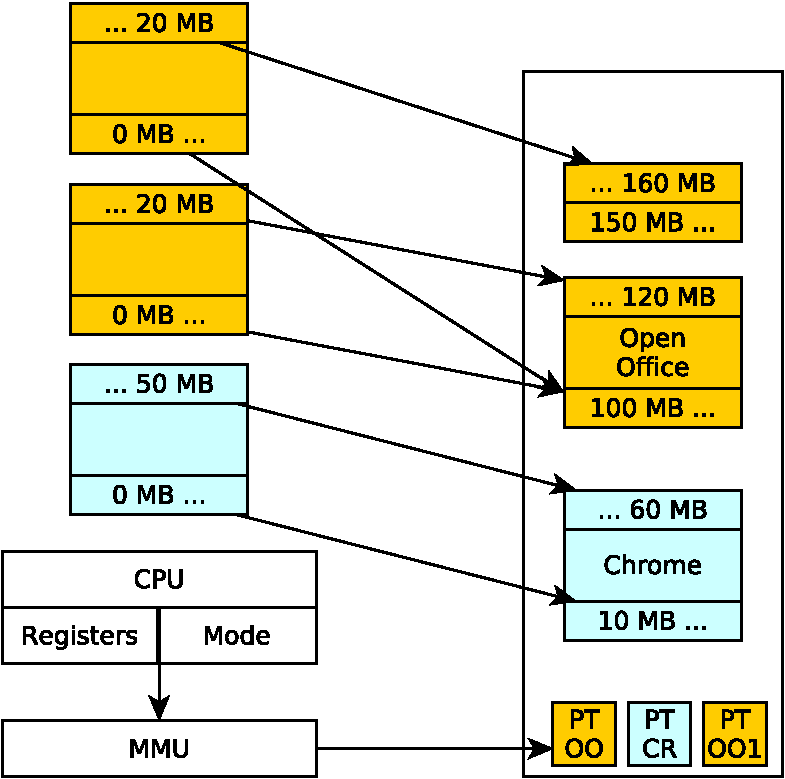
\includegraphics[width=0.6\linewidth]{process2}
\end{frame}

\begin{frame}{Context switch}
    \begin{itemize}
    \item Switch from Open Office to Chrome
    \begin{itemize}
    \item<2-> Change the current PT
    \item<3-> Backup the registers
    \item<4-> Guarantee fairness
    \end{itemize}
    \item<5-> Invoke the OS every x seconds
    \end{itemize}
    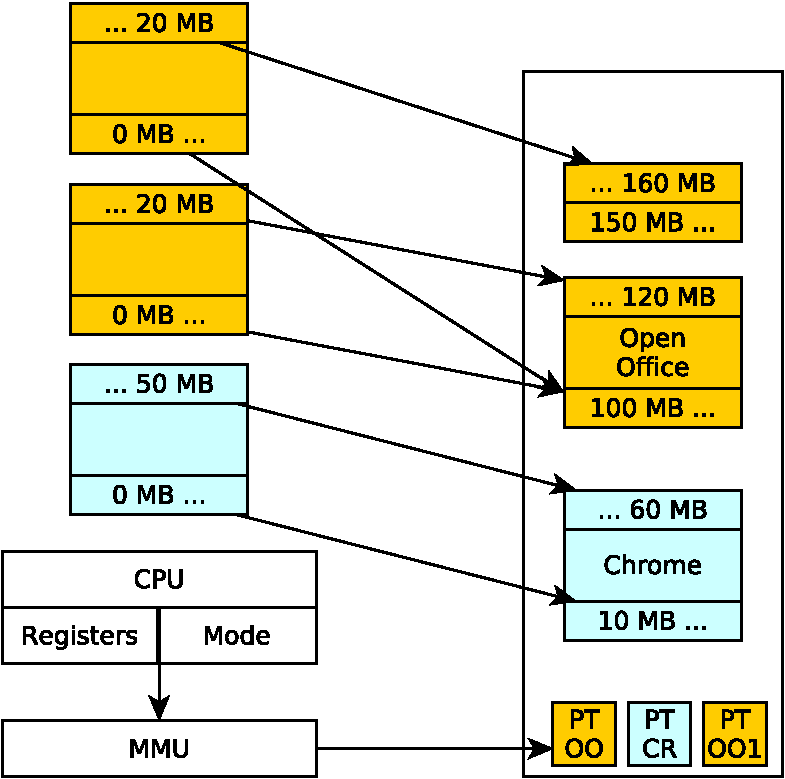
\includegraphics[width=0.3\linewidth]{process2}
\end{frame}

\begin{frame}{Context switch}
  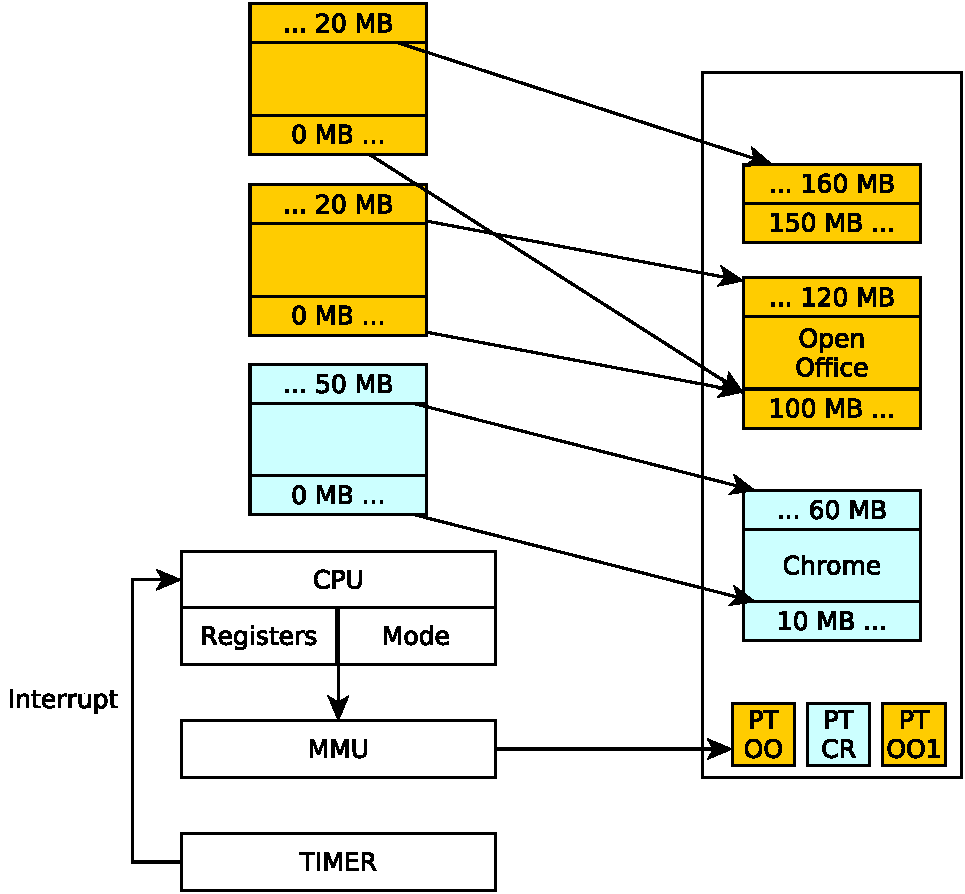
\includegraphics[width=0.7\linewidth]{process3}
\end{frame}

\begin{frame}{Context switch}
  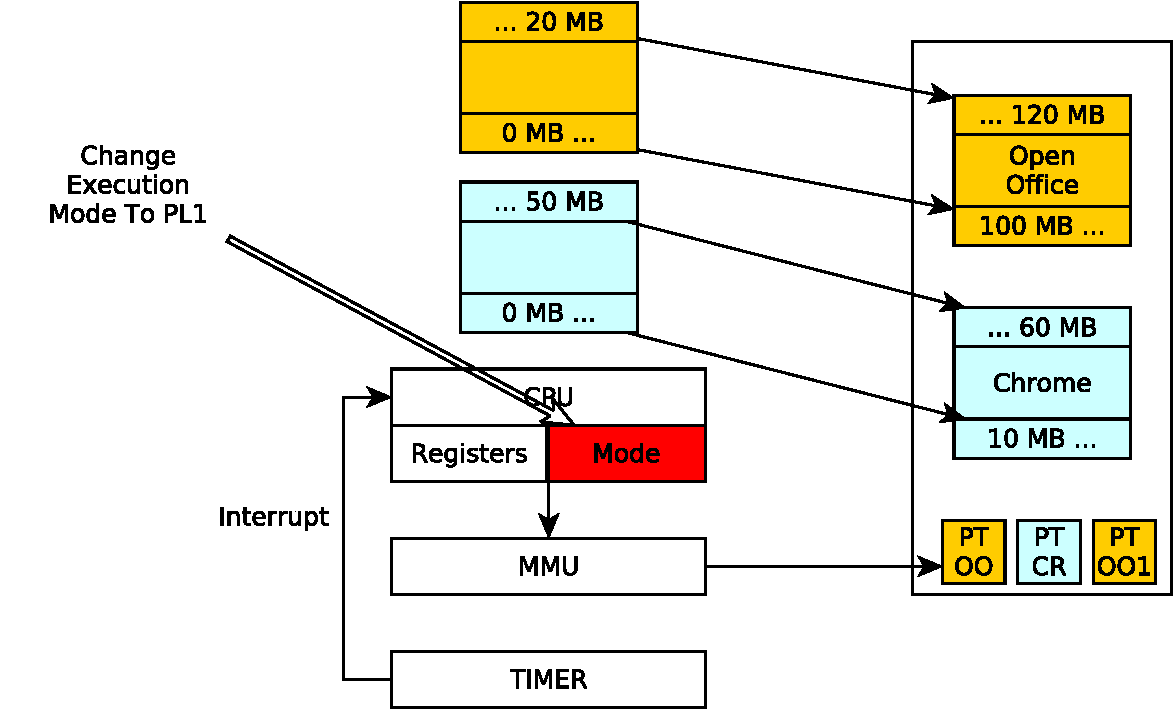
\includegraphics[width=0.7\linewidth]{switch1}
\end{frame}
\begin{frame}{Context switch}
  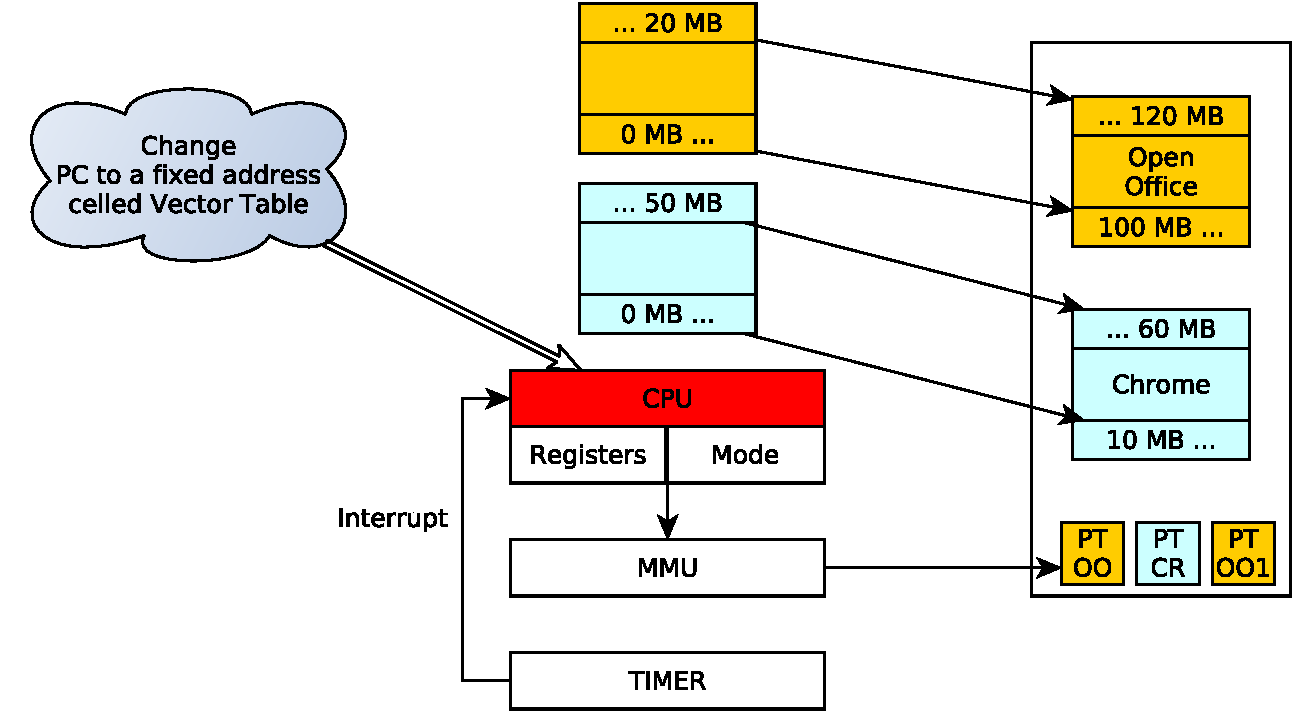
\includegraphics[width=0.7\linewidth]{switch2}
\end{frame}
\begin{frame}{Context switch}
  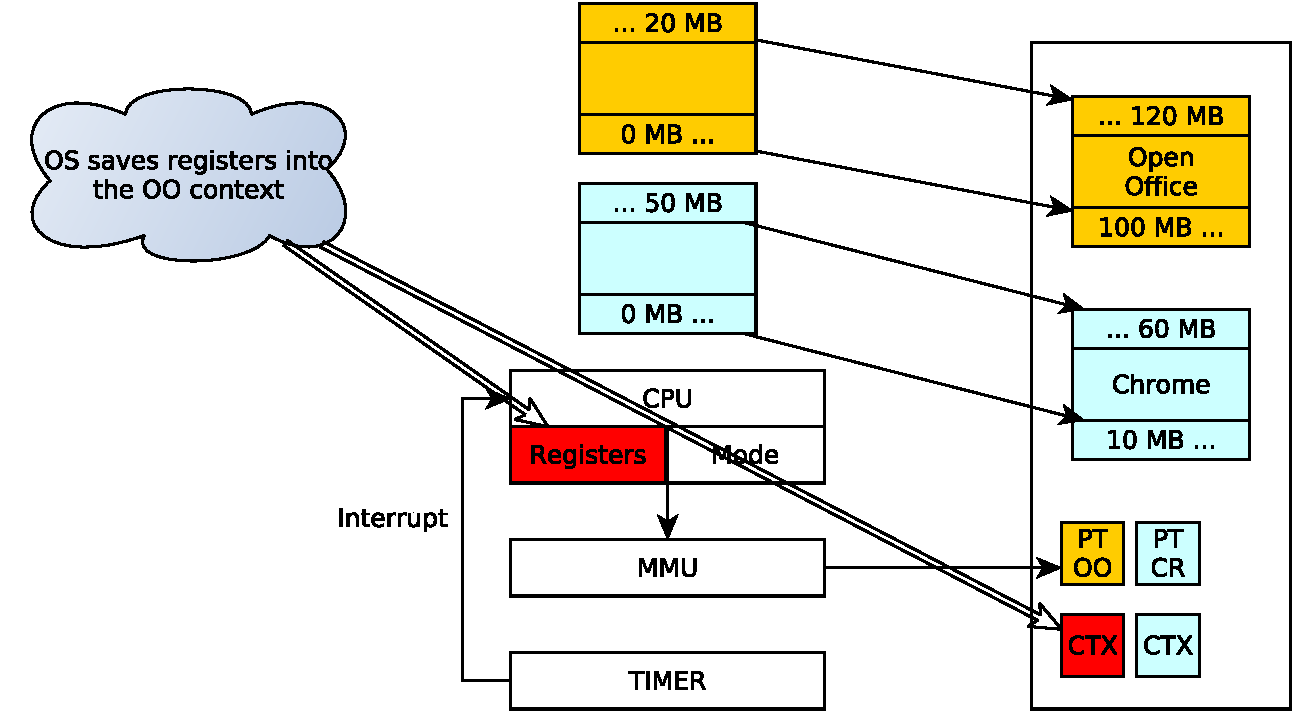
\includegraphics[width=0.7\linewidth]{switch3}
\end{frame}
\begin{frame}{Context switch}
  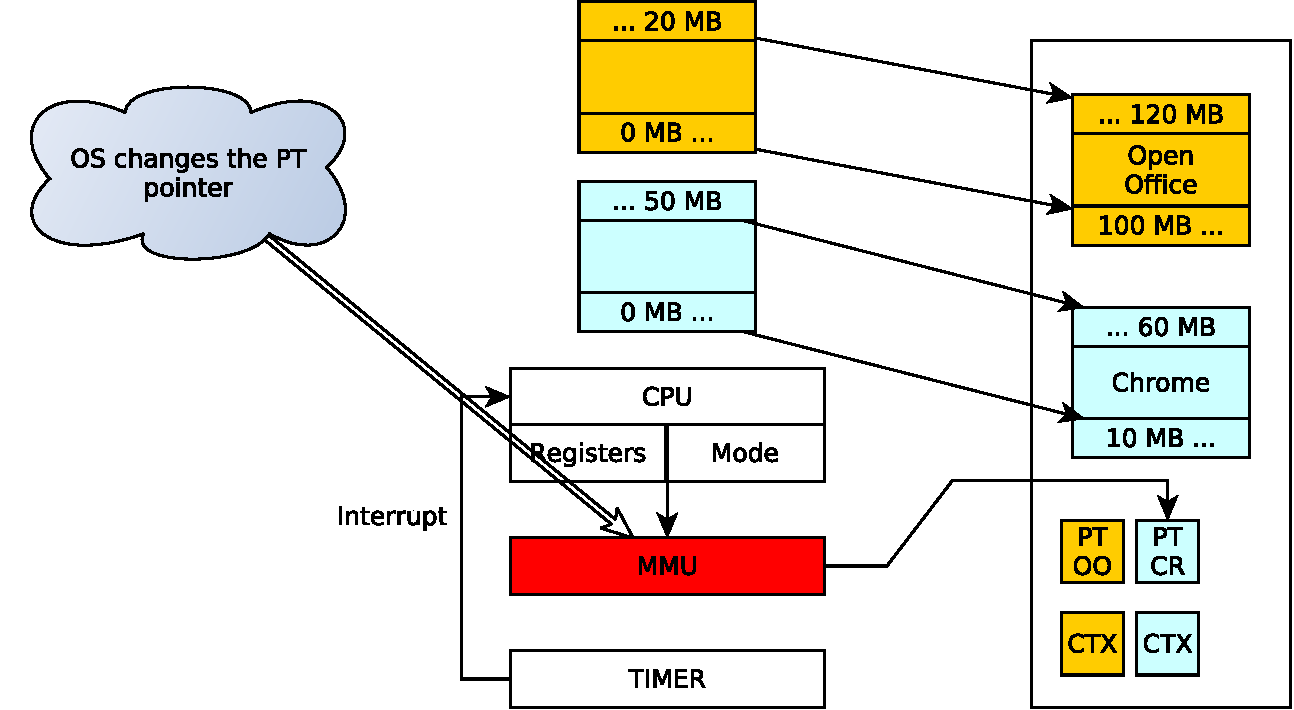
\includegraphics[width=0.7\linewidth]{switch4}
\end{frame}
\begin{frame}{Context switch}
  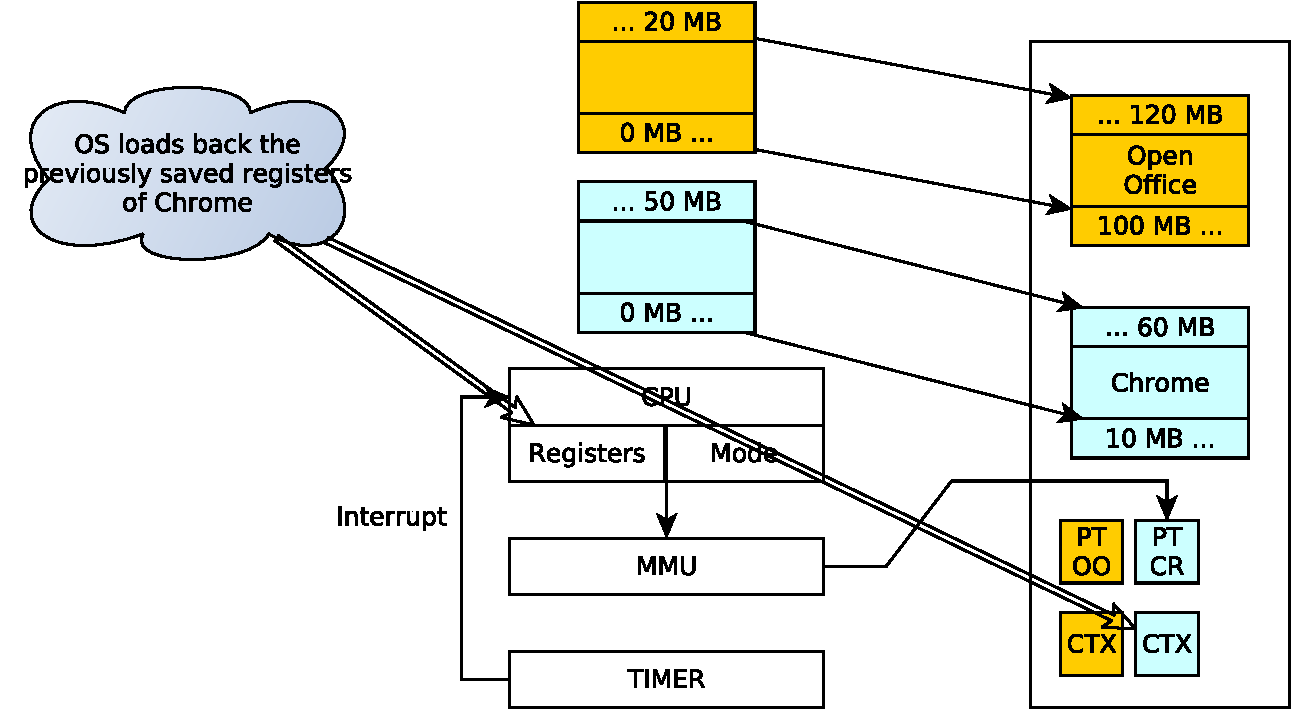
\includegraphics[width=0.7\linewidth]{switch5}
\end{frame}
\begin{frame}{Context switch}
  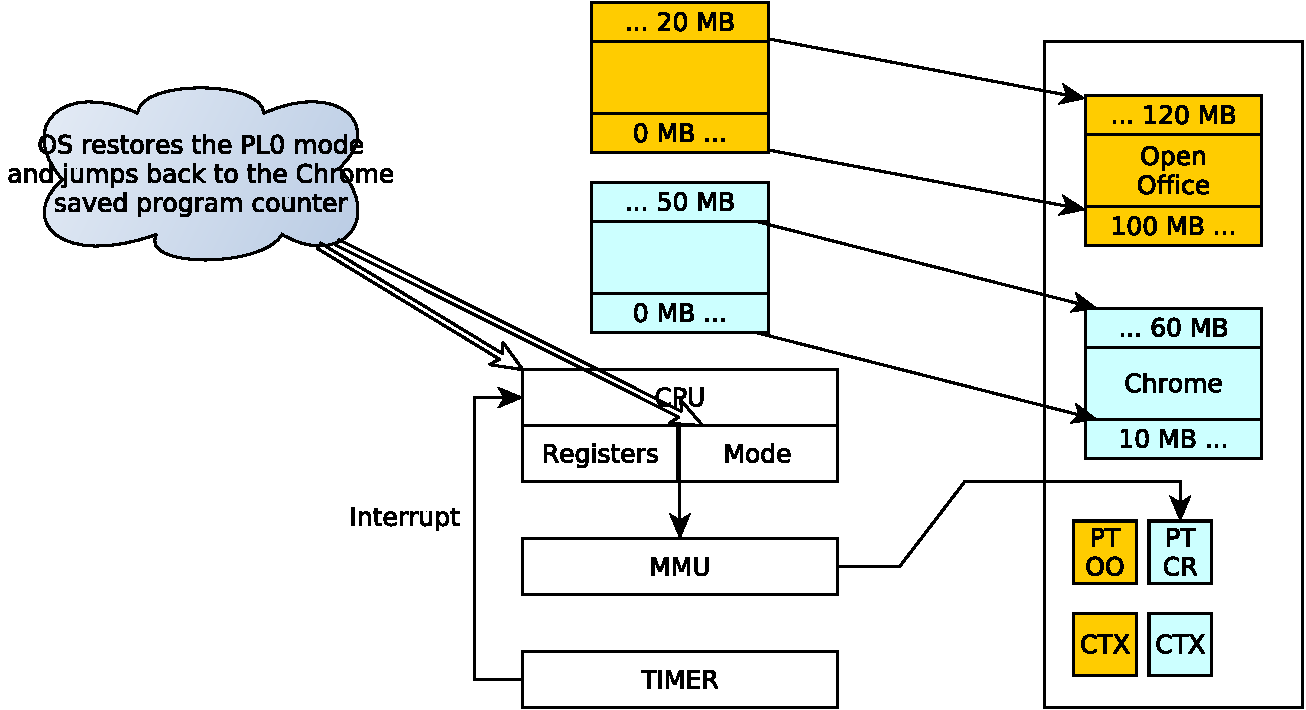
\includegraphics[width=0.7\linewidth]{switch6}
\end{frame}

\begin{frame}{Devices}
  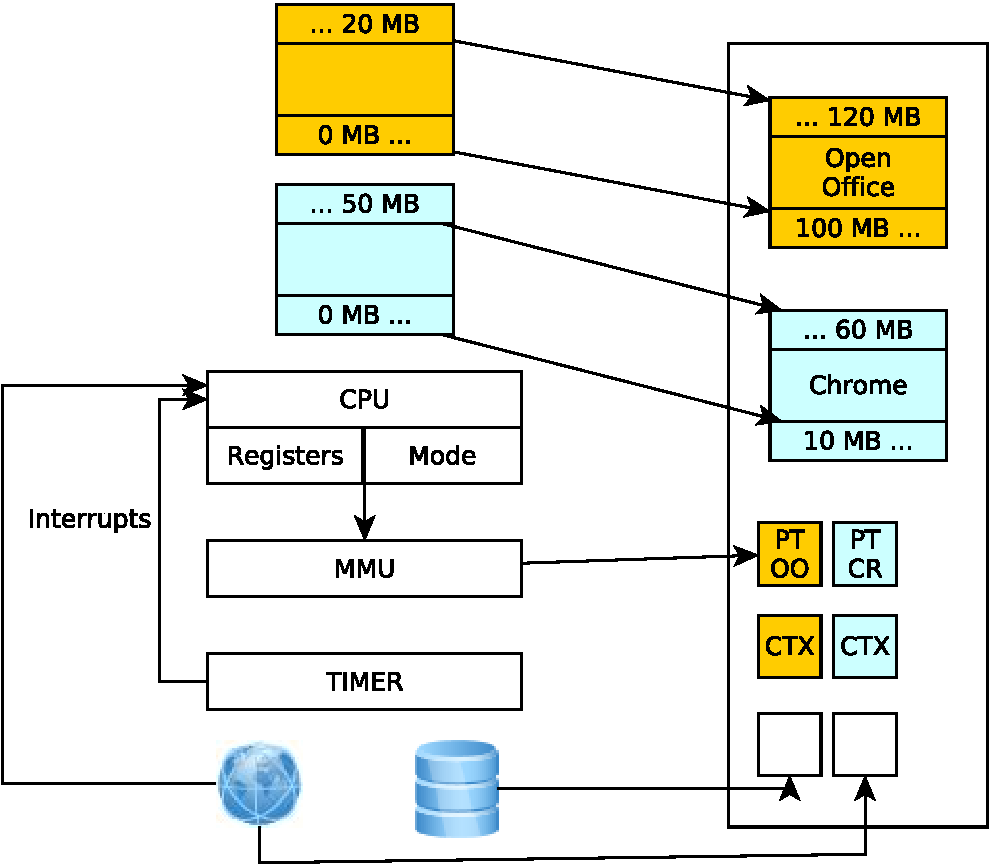
\includegraphics[width=0.7\linewidth]{network}
\end{frame}

\begin{frame}{System calls}
    \begin{itemize}
    \item Request OS services
    \item File management
    \item Device Management
    \item Memory allocation
    \item Process Control
    \item Communication
    \item Print to the terminal
    \item \dots
    \end{itemize}
\end{frame}

\begin{frame}{OS API}
    \begin{itemize}
    \item Syscall low level (and non-portable)
    \item Library or API that sits between normal programs and the
      operating system 
    \item Unix-like: libc, glibc
    \item Windows NT, that API is part of the Native API, in the
      ntdll.dll library
    \item in POSIX: open, read, write, close, wait, exec, fork, exit, mmap
    \end{itemize}
\end{frame}


\end{document}
